%MIT License
%
%Copyright (c) 2018 Chen Wang [https://chenwang.site]
%
%Permission is hereby granted, free of charge, to any person obtaining a copy
%of this software and associated documentation files (the "Software"), to deal
%in the Software without restriction, including without limitation the rights
%to use, copy, modify, merge, publish, distribute, sublicense, and/or sell
%copies of the Software, and to permit persons to whom the Software is
%furnished to do so, subject to the following conditions:
%
%The above copyright notice and this permission notice shall be included in all
%copies or substantial portions of the Software.
%
%THE SOFTWARE IS PROVIDED "AS IS", WITHOUT WARRANTY OF ANY KIND, EXPRESS OR
%IMPLIED, INCLUDING BUT NOT LIMITED TO THE WARRANTIES OF MERCHANTABILITY,
%FITNESS FOR A PARTICULAR PURPOSE AND NONINFRINGEMENT. IN NO EVENT SHALL THE
%AUTHORS OR COPYRIGHT HOLDERS BE LIABLE FOR ANY CLAIM, DAMAGES OR OTHER
%LIABILITY, WHETHER IN AN ACTION OF CONTRACT, TORT OR OTHERWISE, ARISING FROM,
%OUT OF OR IN CONNECTION WITH THE SOFTWARE OR THE USE OR OTHER DEALINGS IN THE
%SOFTWARE.
\documentclass[12pt,a4paper]{Thesis} % Paper size, default font size and one-sided paper

\graphicspath{%
	{./Pictures/}%
	{./Figures/}%
}
\DeclareMathOperator{\Tr}{Tr}
\let\savedegree\degree
\let\degree\relax
\let\savedegree\ref
\let\rem\relax
\usepackage{adjustbox}
\usepackage{amsmath}
\usepackage[amssymb]{SIunits}
\usepackage{amssymb}
\usepackage{multirow}
\usepackage{wrapfig}
\usepackage{subcaption}
\usepackage{mathtools}
\usepackage{lipsum}
\usepackage[ruled,vlined,noresetcount]{algorithm2e}
\usepackage[square, numbers, comma, sort&compress]{natbib} % Use the natbib reference package - read up on this to edit the reference style; if you want text (e.g. Smith et al., 2012) for the in-text references (instead of numbers), remove 'numbers'
% Making url wrap around
\PassOptionsToPackage{hyphens}{url}
\usepackage{hyperref}
\usepackage{url}

\title{\ttitle} % Defines the thesis title - don't touch this

%extra packages
\usepackage{float}
\usepackage{color,soul}               % highlighting text
\usepackage{enumerate}
\usepackage{Styles/mydefs}


\begin{document}

\frontmatter % Use roman page numbering style (i, ii, iii, iv...) for the pre-content pages

\setstretch{1.3} % Line spacing of 1.3
% Define the page headers using the Fr package and set up for one-sided printing

\pagestyle{fancy} % Finally, use the "fancy" page style to implement the FancyHdr headers
\fancyhead{}   %clear all fields
\fancyhead[LO]{\sl{\leftmark}}
\fancyhead[RE]{\sl{\rightmark}}
\fancyhead[LE,RO]{\thepage}


%----------------------------------------------------------------------------------------
%	TITLE PAGE
%----------------------------------------------------------------------------------------

%%% Use \maketitleforreview instead of \maketitle, if you want a PLAIN TITLE PAGE

\maketitle
%\maketitleforreview


% ----------------------------------------------------------------------------------------
% 	ACKNOWLEDGEMENTS
% ----------------------------------------------------------------------------------------

\setstretch{1.3} % Reset the line-spacing to 1.3 for body text (if it has changed)

\acknowledgements{\addtocontents{toc}{\vspace{0.8em}} % Add a gap in the Contents, for aesthetics

I wish to express my greatest gratitude to my advisor.

}


%----------------------------------------------------------------------------------------
%	ABSTRACT PAGE
%----------------------------------------------------------------------------------------

\addtotoc{Abstract} % Add the "Abstract" page entry to the Contents

\pagestyle{fancy} % The page style headers have been "empty" all this time, now use the "fancy" headers as defined before to bring them back

% define the headings for the body of the thesis
\fancyhead{}   %clear all fields
\fancyhead[LO]{\sl{\leftmark}}
\fancyhead[RE]{\sl{\rightmark}}
\fancyhead[LE,RO]{\thepage}

\begin{abstract}
    % 1. The Problem 2. The Issues 3. The Approach 4. The Results 5. The Experiments 6. The Applications
    Distributional word representation such as GloVe and BERT has garnered immense popularity and research interest in recent years due to their success in many downstream NLP applications. However, a major limitation of word embedding is its inability to handle unknown words. To make sense of words that were not present in training, current NLP models use sub-word embedding (obtained via sub-word segmentation algorithms), however, this approach often fails to capture the semantic sense of the word due to words being broken down in a syntactic manner. There has been other approaches to tackle embedding of unknown words using ConceptNet and Recursive Neural Network, but did not enjoy much usage due to their complexities in design. This paper presents a novel solution to generate embedding for OOV using a neural rather than symbolic approach. This approach capitalizes on the existing semantics captured in known words' embedding and trains a simple feed-forward neural network to capture the compositionality function of embedding in their latent space. Linguistic studies have shown that the interested compositionality function is broad and varied, therefore this paper introduces a preliminary study into the compositionality of noun, with focus on certain named entities.  The trained network is able to generate an embedding for an unknown word based on its context words, which can be obtained via crawling of web data. This synthetic embedding can then be incorporated into the embedding matrix of existing application. From our experiments, we can conclude that [include when more results are out]
\end{abstract}

%hack to make ToC starts immediately after abstract
\begingroup
\let\cleardoublepage\clearpage
\tableofcontents %table of content
\listoffigures % Write out the List of Figures
\listoftables % Write out the List of Tables

\mainmatter       % Begin numeric (1,2,3...) page numbering
\pagenumbering{arabic}
\setstretch{1.3}  % Return the line spacing back to 1.3




% Chapter 1

\chapter{Introduction} % Main chapter title
\chaptermark{Introduction}
\label{ch:1_intro} % For referencing the chapter elsewhere, use \ref{Chapter1} 

%----------------------------------------------------------------------------------------
%	SECTION 1
%----------------------------------------------------------------------------------------

\section{Background}

%introduce word embedding, GloVe and BERT

Word embedding as a dense representation of word has received unparalleled popularity among NLP practitioner since its inception compared to other sparse representation such as Brown Cluster or LSA features. Mikolov et al first introduced the word2vec model in 2013 \cite{mikolov2013efficient} and in 2014, GloVe embedding was introduced by Pennington et al \cite{pennington-etal-2014-glove}, GloVe embedding was trained using an architecture similar to CBOW of word2vec, with a slight tweak in objective function, as shown in Figure \fref{fig:word2vec} below. 

\begin{figure}[htbp]
  \centering
    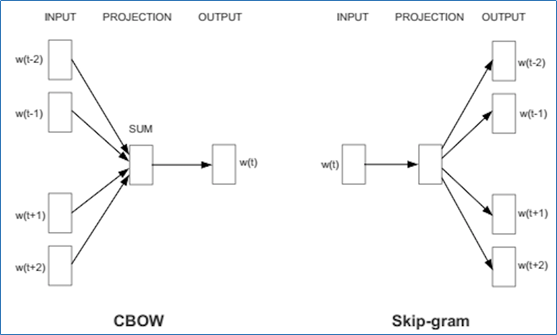
\includegraphics[width=0.85\textwidth]{Figures/Chapter1/word2vec_diagram.png}
  \caption{Architecture of the word2vec model}
  \label{fig:word2vec}
\end{figure}

GloVe authors showed that the ratio of two words' co-occurrence probability (rather than their co-occurrence probabilities themselves) is what conveys information, and that this information is encoded as vector differences. GloVe acquired a lot of traction since they seemed to consistently and significantly outperform standard Distributional Semantic Models. GloVe embedding, however, does not deal well with the problem of polysemy, where the same word has different semantics in different context. This limitation inspires the creation of contextual embedding, with the introduction of transformer models in 2018. Introduced by Vaswani et al in the groundbreaking "Attention is All You Need" paper \cite{DBLP:journals/corr/VaswaniSPUJGKP17}, the Bidirectional Encoder Representations from Transformers (BERT) is a language model that produce tokens which are hugely useful across many NLP tasks. It is distinguished from previous language models by the fact that its learnt representations include context from both sides of the sentences from the architecture that is shown in Figure \fref{fig:bert} below. 

\begin{figure}[htbp]
  \centering
    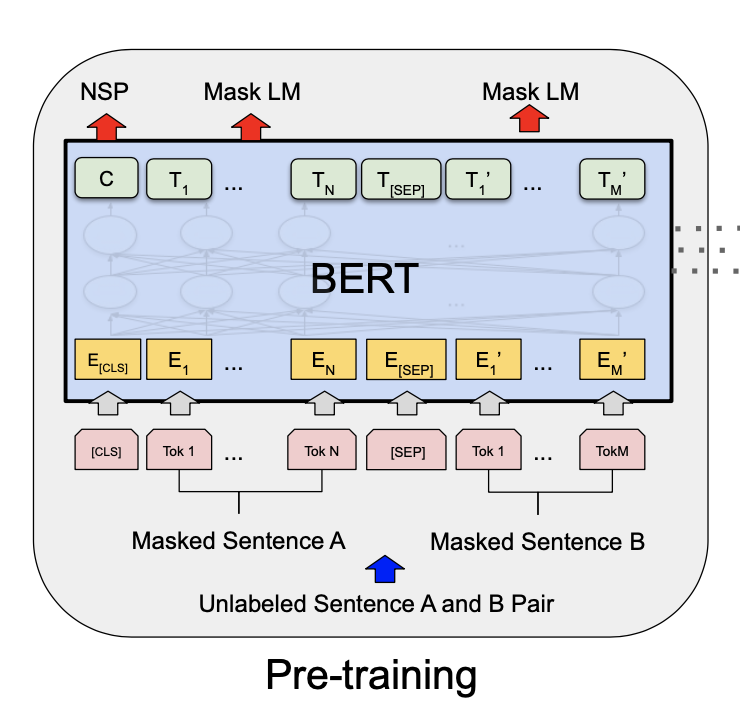
\includegraphics[width=0.85\textwidth]{Figures/Chapter1/bert.png}
  \caption{Bert Architecture}
  \label{fig:bert}
\end{figure}

%introduce the problem of OOV

Despite the major advancement in word embedding research over the last decade, dealing with unknown words still remains as one of the most challenging problems for research and production NLP system. Every NLP model is limited by a fixed-size vocabulary and hence limit the amount of meanings the model can encapsulate about the world. GloVe has a vocabulary size of 40 000 words, and treat any unknown words as OOV while BERT boasts a vocabulary of 30 000 tokens that make uses of sub-words and characters to make sense of an unknown word. As both system are trained on huge corpus of data using tremendous computational power, it is inefficient to retrain the embedding to incorporate new words as NLP systems adapt to the ever-changing environment that they have to operate in. Therefore, in this thesis, we propose a simple method to synthesize a reasonable embedding for a given unknown word. The system is designed to assist mainly in production system, where domain-specific and new words are rare in training corpus but common in production due to high usage from users. An overview of the system supported by this thesis is shown in Figure \fref{fig:workflow} below. 

\begin{figure}[htbp]
  \centering
    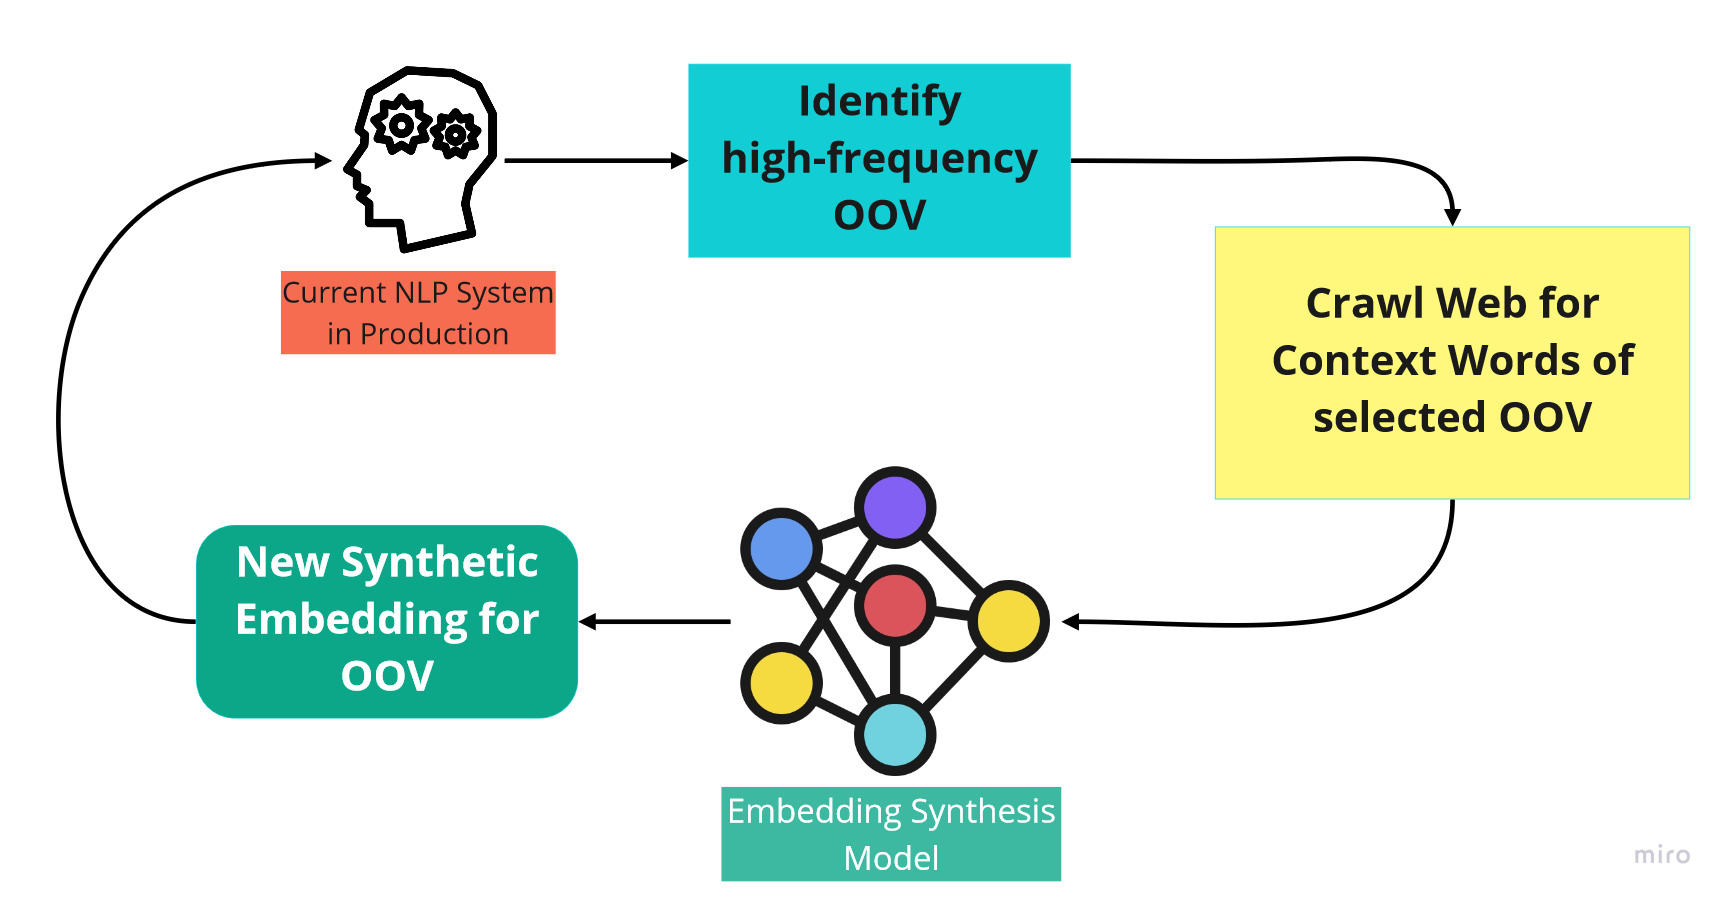
\includegraphics[width=0.85\textwidth]{Figures/Chapter1/workflow.jpg}
  \caption{Workflow of Embedding Synthesis}
  \label{fig:workflow}
\end{figure}

The workflow of the system is as below:

\begin{enumerate}
    \item Current system identify high frequency unknown words that are of high importance
    \item For each word, crawl wiki and related news article about the word 
    \item Pre-process each word and feed it into the embedding synthesis network 
    \item Obtain the new embedding and incorporate it into the current system either via embedding matrix or replacement of embedding
\end{enumerate}

The system is designed to be light-weight and fast to avoid disruption to NLP services in production. The synthetic embedding will help in downstream task to understand unknown words better, with negligible loss. Compared to sub-word segmentation, the synthetic embedding can capture much more semantics information of the word, especially for named entities such as Pfizer. In contrast to pretraining the whole network with OOV corpus, and other sophisticated methods such as ConceptNet ensemble on GloVe \cite{DBLP:journals/corr/VaswaniSPUJGKP17} or Morphology Recurrent Neural Net \cite{luong-etal-2013-better}, the approach in this study is significantly faster and resource-efficient. 

To evaluate the quality of embedding, we follow the suggestion in \cite{schnabel-etal-2015-evaluation}. Relatedness is considered the primary evaluation metric, as analogy is inappropriate in the setting of OOV (which are often rare words). Categorization and Selectional Preference is a feasible metrics but prove to be more challenging to implement. 
% Introduce the 

\newpage

\section{Objectives}

Embedding synthesis is a challenging problem in the research community as there exist no objective metric nor method in creating perfect embedding. Many approaches have been implemented and each of them suffer from their unique limitations, be it resource-heavy or accuracy. In this report, the primary objective is to conduct a study on existing methods and understand their advantages as well as disadvantages. From these understanding, we can create a proof-of-concept model that benefit from the advantages of existing approaches while mitigate as many of the pitfalls as possible. 

The aims of this report are:

\begin{enumerate}
	 \item Design a neural network architecture that are light-weight and is capable of synthesize word embedding
	\item Conduct experiments with different data and hyper-parameters choices on the architecture 
	\item Generate synthetic embedding for a subset of unknown words for GloVe and RoBerta and evaluate these embedding
	\item Provide a method to incorporate existing embedding into system that use GloVe embedding
\end{enumerate}

By securing the above objectives, we will be able to effectively synthesize high-quality embedding in a semi-autonomous manner, thereby greatly reducing the cost and need to retrain the entire network to incorporate meanings of unknown words. As many downstream NLP application such as QA-chatbots and NER suffer from a lack of understanding of unknown words, especially domain-specific named entities, the approach presented in this report can assist NLP engine in production environment by enhancing their capabilities in understanding the text data presented to them by users. 


\newpage

\section{Scope and Assumptions}

The scope of the synthetic embedding generated by the approach in this report is limited to unknown nouns (for training) and named entities of special interest to production such as Pfizer and COVID-19 (for testing). All the related process and methods are developed and tested on online news related to selected keywords. However, it is possible to re-implement the discussed approach in this study, with minor modifications, to adapt it to other unknown words as well. 

The assumptions of the report are:

\begin{enumerate}
    \item Unknown words in NLP production system are typically nouns as they reflect the new trends and phenomena around the world, or cater to services and knowledge in a specific domain. An example of such trend is COVID-19, which has affected many ASR and QA system that are not trained on these words before. Therefore, having a good quality understanding of these words are of special interest as they have potential in enhancing business and services alike. 
    \item The system is designed to trade accuracy and quality reasonably in exchange for a light-weight and fast synthesis method. Cycle time is one of the most crucial factor in user-facing NLP systems, therefore having quick iteration time thanks to fast synthesis can indirectly improve the end-user experience with NLP applications significantly. Additionally, as embedding is used as an input to downstream tasks, a slight reduction in accuracy is acceptable for well-tuned system as they are able to make maximum use of the information captured inside the embedding. 
\end{enumerate}

\newpage

\section{Report Organization}

This report is sectioned into five chapters as follow:
\begin{itemize}
    \item Chapter 1 presents a brief introduction into the project and its background, followed by the project's objectives, scope and assumptions
    \item Chapter 2 focuses on the literature review of existing approaches to synthesize word embedding, followed by a brief discussion on metrics suited for the objective and inspiration to the current approach
    \item Chapter 3 proposes the system design, the methodology and specifications of the system
    \item Chapter 4 details the implementation of each individual component of the system, from data curation and ingestion to output
    \item Chapter 5 presents the experiments results and evaluate its efficacy 
    \item Chapter 6 explores briefly different properties of the synthetic embedding that are useful for production, and gives several recommendations to modifying existing approach
    \item Chapter 7 gives a conclusion to the report and explore possible future work
\end{itemize}



% Chapter 2

\chapter{Literature Review}
\chaptermark{Literature Review}

This section presents a survey of existing approaches to deal with OOV as well as their advantages and disadvantages. The main approaches can be broadly divided into (1) sub-word segmentation, (2) fine tuning on better corpus, and (3) other novel methods. By examining the various different approaches to dealing with unknown words, we gain a better understanding of the properties of word-embedding in their latent space and the time and memory complexity of each method's implementation. From there, we hope to combine the insights and groundwork of these studies to come up with an implementation best suited for our specifications. 

\section{Sub-word Segmentation}

Segmentation, in general, is a technique to separate an input text into useful components for analysis. Before sub-word segmentation becomes popular, word segmentation was widely adopted in research and production field. However, it requires a huge vocabulary size (approximately 70000 words for English) and thus pose a huge constraints in training and storing models.Further more, many tokens overlap, such as 'look' and 'looks', which do not provide meaningful information to NLP models. Character-level segmentation and word-char hybrid models were introduced in \cite{DBLP:journals/corr/LuongM16}, where the character model evaluated on the \emph{newstest2015} NMT dataset achieved competitive BLEU-score with significantly smaller vocabulary size. However it is difficult to train and tune these character level models due to its long convergence (3 months compared to 3 weeks for a similar word-level model \cite{DBLP:journals/corr/LuongM16}. To tackle these issues, \cite{sennrich-etal-2016-neural} introduced the concept of segmenting words into sequences of sub-word units to provide a more meaningful representation within a reasonable vocabulary size. A brief overview of the aforementioned approaches is presented in table \tref{tab:segmentation} for illustration.

\begin{table}
	\centering
	\begin{tabular}{cc}\toprule
		Input  & \'Cooked\' \\\midrule
		Word level & ['Cooked']\\
		Char level & ['C','o','o','k','e','d']\\
		Sub-word   & ['Smoke','\#ed']\\
		\bottomrule
	\end{tabular}
	\caption{Word, Character and Sub-word segmentation}
	\label{tab:segmentation}
\end{table}

Based on the idea of segmenting text input into meaningful token within a reasonable vocabulary size, many sub-word approaches have emerged and are adopted across the field. In this report, we will focus on the 4 main sub-word techniques (and its variants) that are most widely used and are most popular in NLP: 

\begin{enumerate}
	\item Byte-Pair-Encoding (BPE)
	\item WordPiece 
	\item Unigram Language Model (ULM)
	\item FastText 
\end{enumerate}

\subsection{Byte-Pair-Encoding} 

\subsection{WordPiece}

\subsection{Unigram Language Model}

\subsection{FastText} 

2.1.2 BPE

https://aclanthology.org/P16-1162/ 

2.1.3 FastText 

https://paperswithcode.com/paper/enriching-word-vectors-with-subword 

2.2 Retraining

train on Singlish (medium) 

2.3 ConceptNet

using the conceptnet and ppdb to produce wordvec of .... 

2.4 Recursive NN 

https://nlp.stanford.edu/~lmthang/morphoNLM/ 



2.4 Properties of Word Embeddings 

Vector additivity 



\input{Chapters/3_proposed_approach}
\endgroup


\label{Bibliography}
\setstretch{1}
\bibliographystyle{unsrtnat}
\bibliography{References/ref}

\end{document}
